\documentclass{beamer}

\usepackage{beamerthemesplit}

\title{Structured ASIC}
\subtitle{ }
\subtitle{CMPE584 - Reconfigurable Computing}
\author{Onur \"Ozkol}
\date{December - 2009}

\begin{document}

\frame{
  \titlepage
}

\section{Introduction}
\subsection{What is a structured ASIC?}
\frame
{
  \frametitle{What is a structured ASIC?}
  \begin{itemize}
  \item It is an intermediate technology between ASIC and FPGA.
  \item It is a pre-configured (or hardwired) FPGA application.
  \end{itemize}
  \begin{figure}[H]
  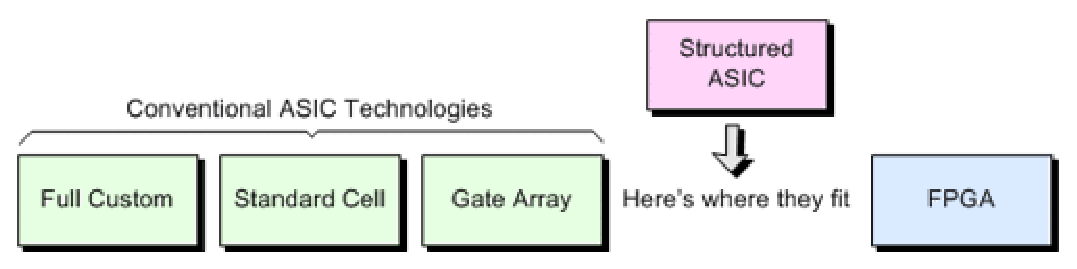
\includegraphics[height=20mm]{images/where_fit_asic.eps}
  \end{figure}
}

\frame
{
  \frametitle{What is a structured ASIC?}
  Simply it is metal-layer configurable ASIC.
  \begin{figure}[H]
  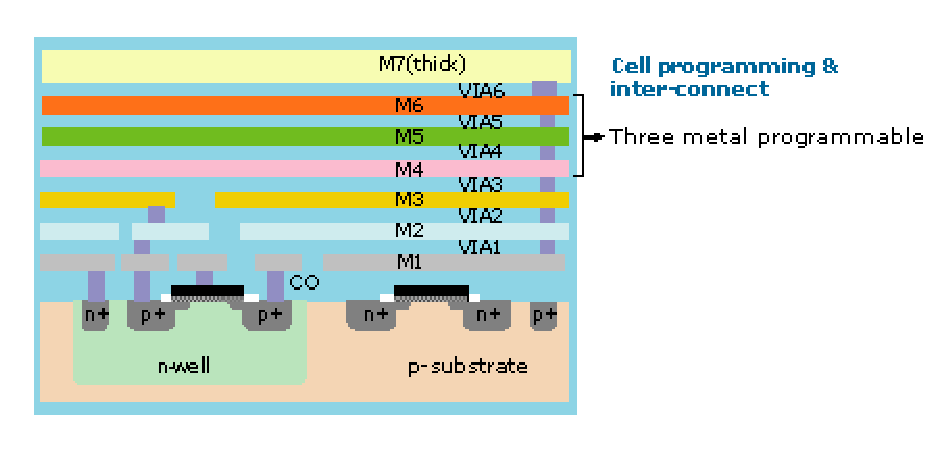
\includegraphics[height=50mm]{images/inside.eps}
  \end{figure}
}

\subsection{Acronyms}
\frame
{
  \frametitle{Acronyms used in this presentation}
  \begin{itemize}
  \item SEU: Single Event Upset is a change of state caused by a high-energy particle strike to a sensitive node in a micro-electronic device, such as in a microprocessor, semiconductor memory, or power transistors.
  \item NRE: Non-recurring engineering (NRE) refers to the one-time cost of researching, developing, designing, and testing a new product. 
  \item S-ASIC: Structured Application Specific Integrated Circuit
  \item ASSP: Application Specific Standart Products
  \end{itemize}
}

\section{Uses}
\subsection{Uses}
\frame
{
  \frametitle{Uses of Structured ASIC}
  \begin{itemize}
  \item It is used for reducing SEU (Invented then)
  \item It is used for easy prototyping.
  \item It is used for lowering costs for low and mid volume application. 
  \item It is used for when something needed between FPGA and ASIC.
  \end{itemize}
}

\subsection{Benefits}
\frame
{
  \frametitle{Benefits}
  \begin{itemize}
  \item It offers higher performance, a characteristic of ASIC,
  \item It offers lower power requirements, a characteristic of ASIC 
  \item It offers low NRE cost, a characteristic of FPGA. 
  \end{itemize}
}

\section{Architectures}
\subsection{Inside S-ASIC}
\frame
{
  \frametitle{Inside S-ASIC}
  \begin{columns}
  \begin{column}[l]{5cm}
  Topview
  \begin{figure}[H]
  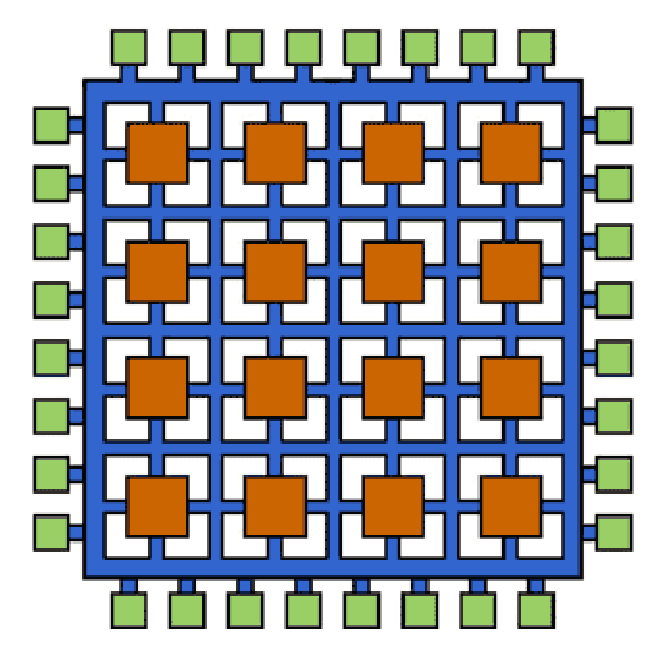
\includegraphics[height=40mm]{images/structured.eps}
  \end{figure}
  \end{column}
  \begin{column}[r]{5cm}
  Layers
  \begin{figure}[H]
  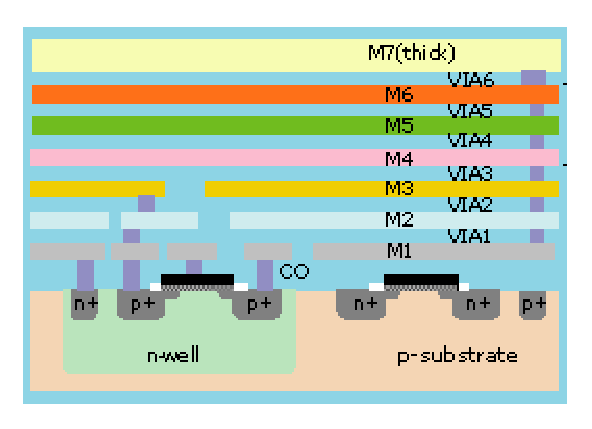
\includegraphics[height=40mm]{images/inside2.eps}
  \end{figure}
  \end{column}
  \end{columns}
}

\subsection{Granularity}
\frame
{
  \frametitle{Granularity}
  Granularity defines the minimum configurable unit.
  \begin{itemize}
  \item Fine-grained requires many connection in and out of a structured element.
  \item Coarser granularities reduce connections but decreases the element functionality. 
  \end{itemize}
}

\frame
{
  \frametitle{Fine Grain}
  Fine-grained asics are configurable as resistors, caps, or basic logic gates.
  \begin{figure}[H]
  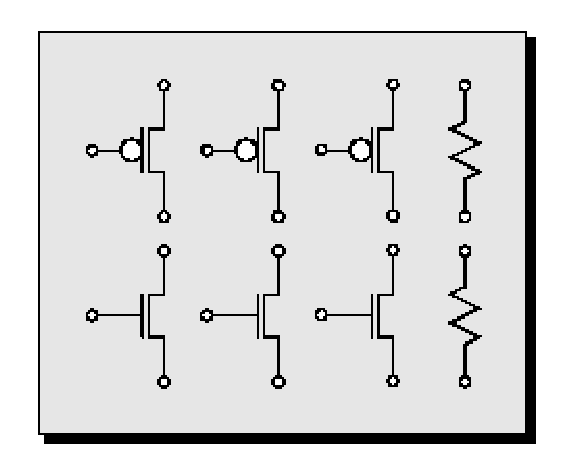
\includegraphics[height=40mm]{images/fine_grained.eps}
  \end{figure}
}

\frame
{
  \frametitle{Mid Grain}
  Mid-grained(sometimes coarse-grained) asics are configurable as blocks, like FPGA blocks.
  it shows both memory and sequantial element properties.
  \begin{figure}[H]
  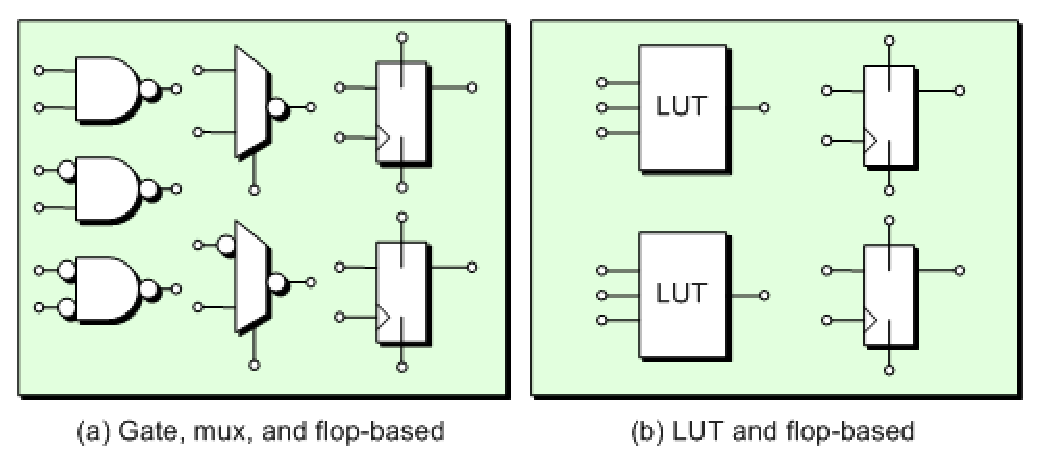
\includegraphics[height=40mm]{images/mid_grained.eps}
  \end{figure}
}

\frame
{
  \frametitle{Coarse Grain}
  Coarse-grained ones are configurable like cpu and some pheripherals are enabled or disabled.
  \begin{figure}[H]
  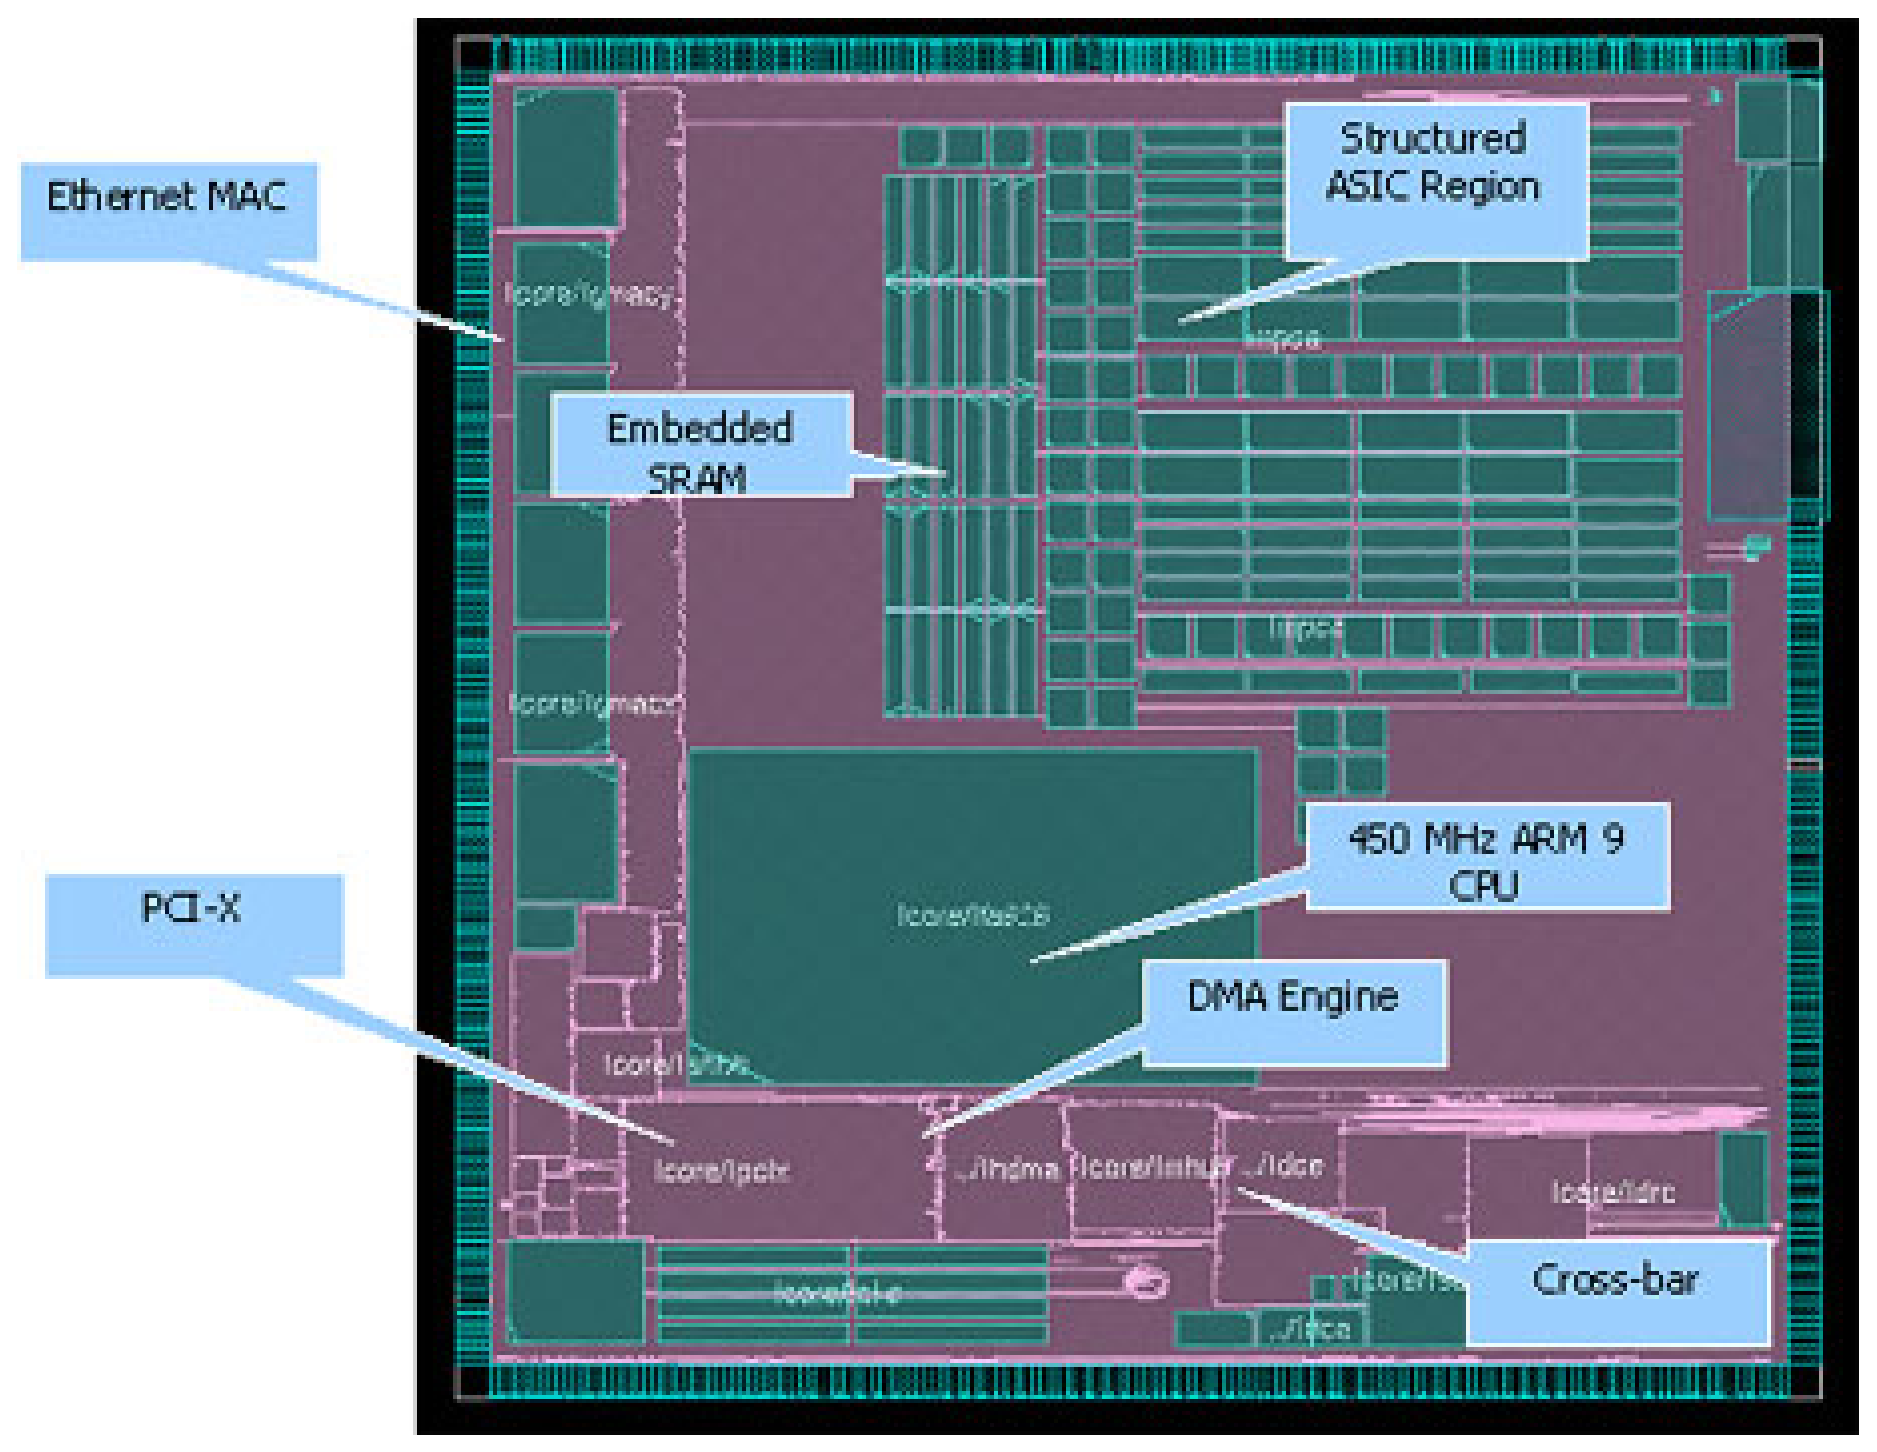
\includegraphics[height=50mm]{images/coarse_grained.eps}
  \end{figure}
}

\subsection{Clock Network}
\frame
{
  \frametitle{Clock Network}
  Nearly all types of S-ASIC contain a clock network.
  \begin{itemize}
  \item Some global clocks, and more local clocks.
  \item Helps to meet timing requirements easily. 
  \end{itemize}
}


\section{Comparison}
\subsection{Advantages}
\frame
{
  \frametitle{Advantages}
  \begin{itemize}
  \item Lot more! Some importants are,
  \item Structured ASIC combines the advantages of both ASIC and FPGA.
  \item Power efficiency, better performance.
  \item Low turn-over rate while developing ASIC.
  \item S-ASIC devices has a clock network, ASIC doesnt.
  \item 1:3:12 power consumption ratios (ASIC:S-ASIC:FPGA)
  \item FPGA to ASIC conversion comes with smaller packaging.
  \item More secure, against reverse engineering, or hacking.
  \item Hybrid ASICs very good option for projects with requirements are not defined well or changing.
  \end{itemize}
}

\subsection{Disadvantages}
\frame
{
  \frametitle{Disadvantages}

  \begin{itemize}
  \item It is not fully customizable like ASIC.
  \begin{itemize}
  \item We cannot tweak, customize or modify unit smaller than vendor determined.
  \item For example, we cannot change W values of a transistor group. 
  \end{itemize}
  \item It is not field programmable, it is one-time programmable when manufacturing. 
  \item You may need to redesign or change the design methodology when FPGA to S-ASIC
  \end{itemize}
}

\subsection{Comparison to ASIC and FPGA}
\frame
{
  \frametitle{S-ASIC combines advantages of both technologies}
  \begin{columns}
  \begin{column}[l]{5cm}
  FPGA
  \begin{itemize}
  \item {\color{green!40!gray}Easy to design}
  \item {\color{green!40!gray}Short development time}
  \item {\color{green!40!gray}Low NRE Cost}
  \item {\color{red}Design size is limited}
  \item {\color{red}Design complexity limited}
  \item {\color{red}Performance limited}
  \item {\color{red}High power consumption}
  \item {\color{red}High per-unit cost}
  \item {\color{red}SEU sensitive}
  \end{itemize}
  \end{column}
  \begin{column}[r]{5cm}
  ASIC
  \begin{itemize}
  \item {\color{red}Difficult to design}
  \item {\color{red}Long development time}
  \item {\color{red}High NRE costs}
  \item {\color{green!40!gray}Support large designs}
  \item {\color{green!40!gray}Support complex designs}
  \item {\color{green!40!gray}High performance}
  \item {\color{green!40!gray}Low power consumption}
  \item {\color{green!40!gray}Low per-unit cost}
  \item {\color{green!40!gray}lower SEU sensivity}
  \end{itemize}
  \end{column}
  \end{columns}
}

\frame
{
  \frametitle{Comparison to ASIC and FPGA}
  \begin{figure}[H]
  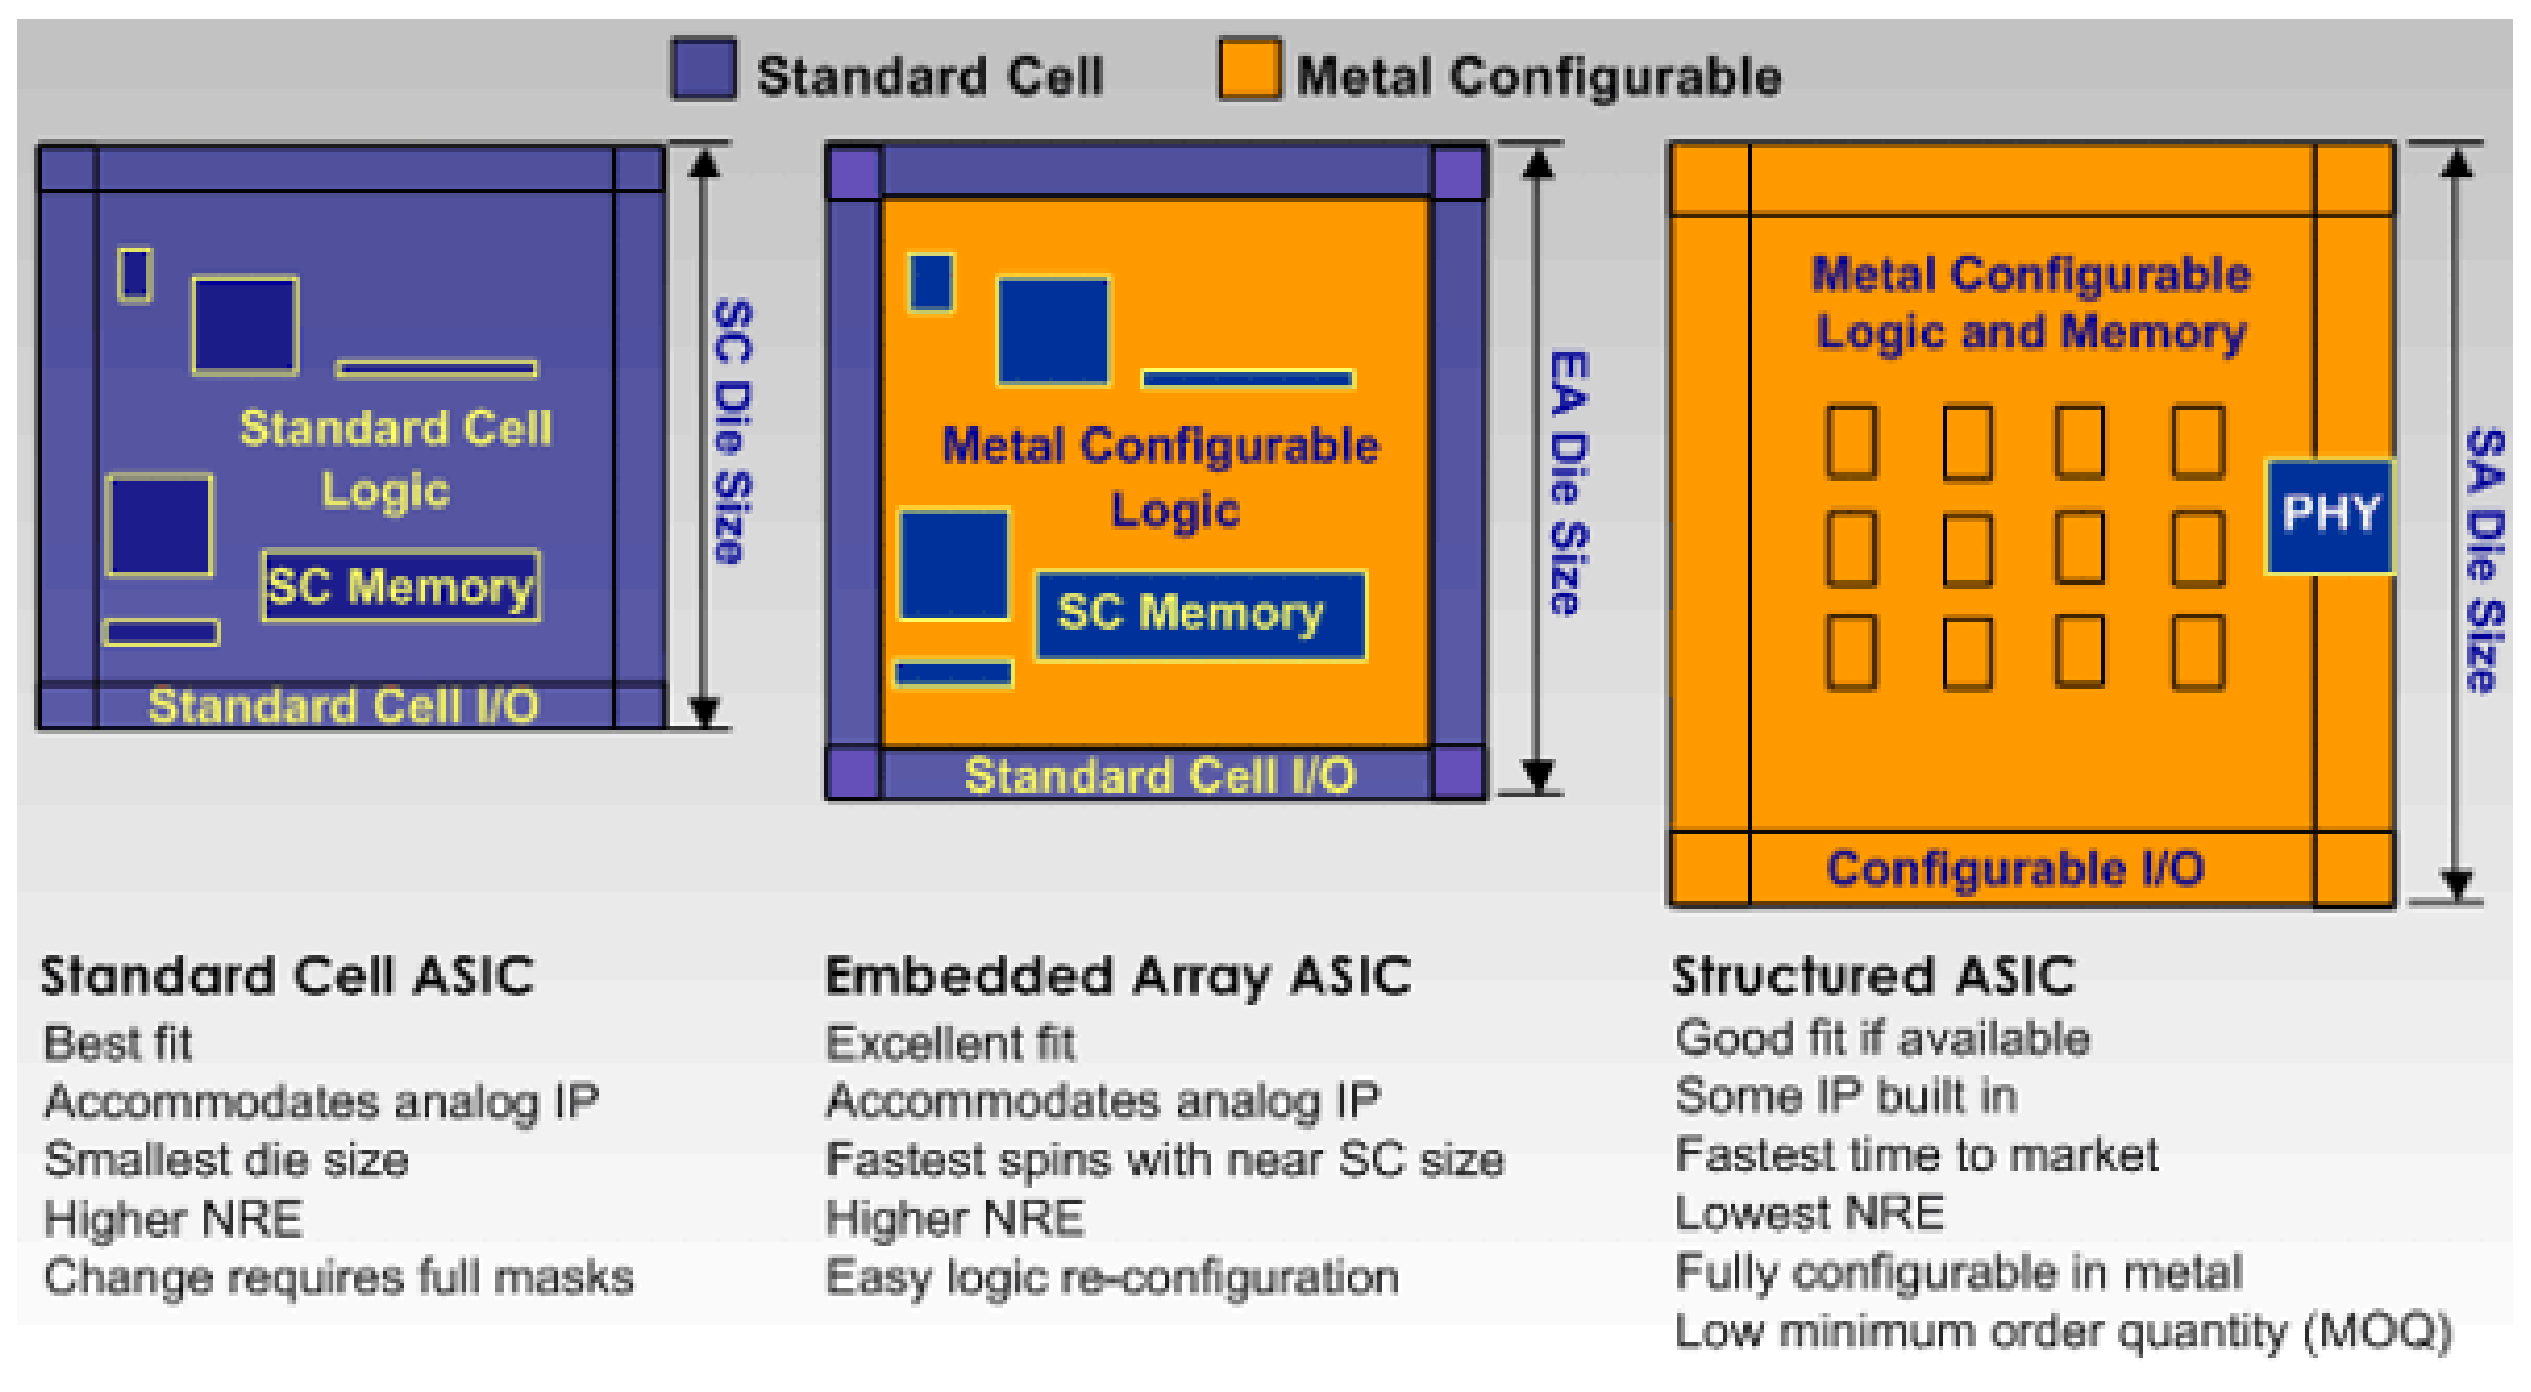
\includegraphics[height=60mm]{images/comparison_to_asic.eps}
  \end{figure}
}


\section{Vendors/Technologies}
\subsection{Structured ASIC Companies}
\frame
{
  \frametitle{Structured ASIC Companies}
  \begin{figure}[H]
  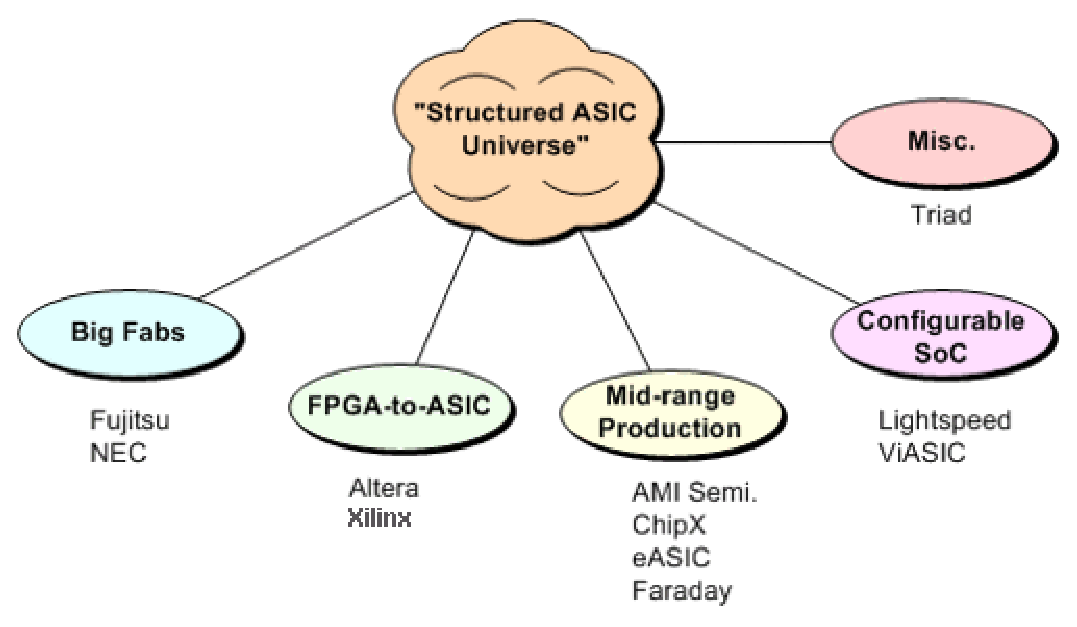
\includegraphics[height=60mm]{images/vendors.eps}
  \end{figure}
}

\subsection{Big Fabs}
\frame
{
  \frametitle{Big Fabs}
  \begin{itemize}
  \item They also provide (and require) their tools.
  \item When a new process technology appears, that is generally tested by producing S-ASIC or FPGA. 
  \item Because of it is not effective in high volumes, LSI and Fujitsu abandoned.
  \end{itemize}
}

\subsection{FPGA-to-ASIC}
\frame
{
  \frametitle{Xilinx EasyPath}
  \begin{itemize}
  \item Please note, Xilinx is a fabless company, which contracts to Samsung and TSMC.
  \item Almost all xilinx devices is supported.(not all)
  \item 3 Months production time.
  \end{itemize}
  \begin{figure}[H]
  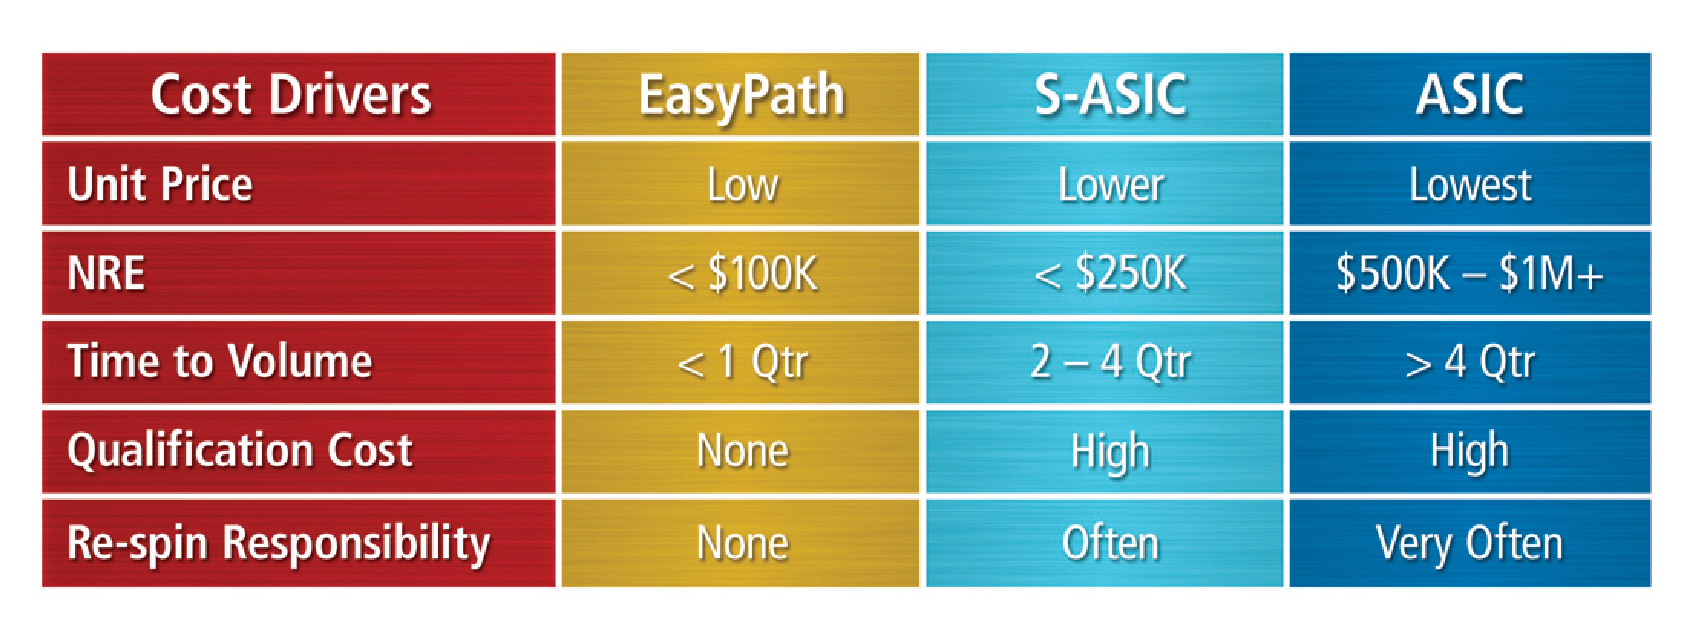
\includegraphics[height=35mm]{images/easypath.eps}
  \end{figure}
}

\frame
{
  \frametitle{Altera Hardcopy}
  \begin{columns}
  \begin{column}[l]{6cm}
  \begin{itemize}
  \item \%5 of total revenue
  \item One tool, One methodology, One manufacturer
  \item Downto 40nm process
  \item Upto 12 Million gates in a device
  \item May Include Altera 6.5gbps transreceivers
  \end{itemize}
  \end{column}
  \begin{column}[r]{6cm}
  \begin{figure}[H]
  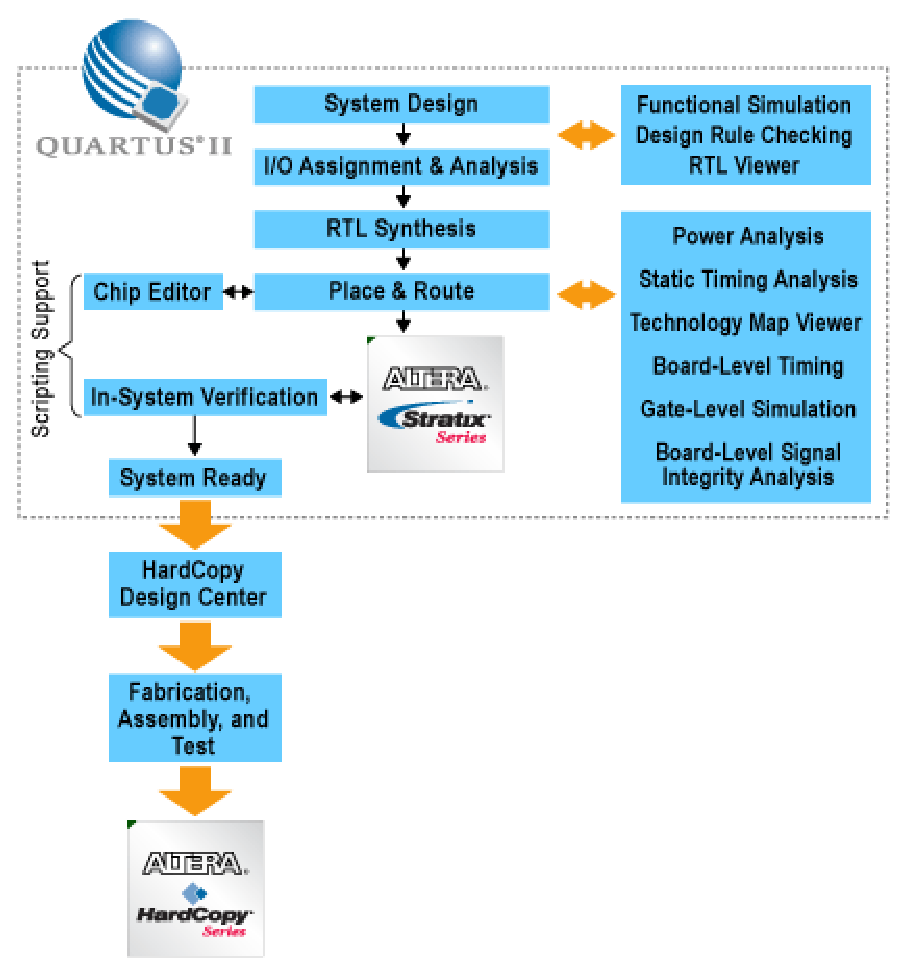
\includegraphics[height=58mm]{images/altera-hardcopy.eps}
  \end{figure}
  \end{column}
  \end{columns}
}

\subsection{Mid-range Production}
\frame
{
  \frametitle{Mid-range Production}
  \begin{itemize}
  \item Each company have different approach.
  \item Real S-ASIC companies!
 
  \item chipx \url{http://www.chipx.com}
  \begin{itemize}
  \item Coarse grain ASIC products, with clocks, memory controller, buses are ready
  \end{itemize}

  \item Faraday \url{http://www.faraday-tech.com}
  \begin{itemize}
  \item Ready to deploy SoC also with SW.
  \end{itemize}

  \item easic \url{http://www.easic.com}
  \begin{itemize}
  \item FPGA vendor like but in mid-volumes only.
  \item Developed its tools and IDE, available free.
  \end{itemize}

  \end{itemize}
}

\subsection{Configurable SOC}
\frame
{
  \frametitle{Configurable SOC}
  \begin{itemize}
  \item Actually these companies provides ASIC with a small configurable area.
  \item They are simply SoC development contractors.
  \item Less configurable devices. Having 1 - 2 metal layer programmable.  
  \end{itemize}
}


\subsection{Misc}
\frame
{
  \frametitle{Misc}

  \begin{itemize}
  \item Other companies that doesnt fit any category.

  \begin{itemize}
  \item triad \url{http://www.triad.com}
  \item ASIC products, with pre-sythesized op-amps, filters, DACs
  \item FPGA like granularity with more analog devices.
  \end{itemize}
  \end{itemize}

}

\section{Conclusion}
\subsection{Market Status}
\frame
{
  \frametitle{Market Status}
  \begin{itemize}
  \item Some people thinks it is a revolution
  \item However, some companies abandoned it. because,
  \begin{itemize}
  \item	Flow issues
  \item Over promising
  \item Poor execution
  \item but many companies still in operation.
  \end{itemize}
  \item Highly innovative, low and mid volume designs use it.
  \item Aerospace/Defense companies uses it.
  \item The way of easy FPGA-to-ASIC conversion.
  \item EDA tools for S-ASIC should be developed.
  \end{itemize}
}

\subsection{References}
\frame[shrink=50]
{
  \frametitle{References}
  \begin{enumerate}
  \item	  \url{http://en.wikipedia.org/wiki/Application-specific_integrated_circuit}
  \item	  \url{http://en.wikipedia.org/wiki/Application_specific_standard_product}
  \item	  \url{http://www.soccentral.com/results.asp?CatID=488&EntryID=22566}
  \item	  \url{http://www.soccentral.com/results.asp?CatID=488&EntryID=22567}
  \item	  \url{http://www.soccentral.com/results.asp?CatID=488&EntryID=19387}
  \item	  \url{http://www.soccentral.com/results.asp?CatID=488&EntryID=15885}
  \item	  \url{http://www.mil-embedded.com/articles/id/?2872}  
  \item	  \url{http://www.faraday-tech.com/html/products/structuredASIC.html}
  \item	  \url{http://www.eetimes.com/industrychallenges/silicon/showArticle.jhtml?articleID=21401237}
  \item	  \url{http://www.chipx.com/cx6100-structured-asic.html}
  \item	  \url{http://www.newelectronics.co.uk/article/18880/Whatever-happened-to-structured-asics-.aspx}
  \item	  \url{http://www.altera.com/products/software/flows/asic/qts-structured_asic.html}
  \item	  \url{http://www.altera.com/products/devices/hardcopy-asics/about/hrd-index.html}
  \item	  \url{http://www.eetimes.com/story/OEG20020325S0060}
  \item	  \url{http://www.techonline.com/article/192200241}
  \item	  \url{http://www.electronicsweekly.com/Articles/2004/10/26/33416/The-promise-of-structured-Asic.htm}
  \item	  \url{http://www.fpgajournal.com/fpgajournal/feature_articles/20091215-myopia/}
  \item	  \url{http://findarticles.com/p/articles/mi_m0GZQ/is_41_45/ai_n8968679}
  \item	  \url{http://viasic.com/}
  \end{enumerate}
}

\subsection{Thank you}
\frame
{
  \frametitle{Thank you}
  Questions ?
}

\end{document}
